\documentclass[aspectratio=43,unicode,10pt]{beamer}
\usetheme{ttipresentation}

\usepackage{luatexja}
\usepackage{luatexja-fontspec}
\usepackage{graphicx}
\usepackage{multicol}

\setmainjfont{ipagp.otf}
\beamertemplatenavigationsymbolsempty

\newcommand{\itemtitle}[1]{\textbf{#1}\\}
\newcommand{\fire}[1]{\textcolor{red}{\textbf{#1}}}
%\newcommand{\freeze}[1]{\textcolor{blue}{\textbf{#1}}}
\newcommand{\then}{\textcolor{ttiblue}{\textbf{⇒}}\hspace{1ex}}
\newcommand{\good}{\textcolor{orange}{\textbf{◎}}\hspace{1ex}}
\newcommand{\arrow}{\textcolor{ttiblue}{\textbf{→}}\hspace{1ex}}
\newcommand{\mb}[1]{\mathbf{#1}}
\newcommand{\arrowed}[1]{\vec{\mathbf{#1}}}


\newcommand{\thetitle}{レーティング予測によるフォントに基づくレビュー解析}
\title{\thetitle}
\institute{知能数理研究室}
\author{外山洋太、三輪誠、佐々木裕}
\date{\today}


\newcommand{\bigger}{\Large}

\begin{document}

\begin{frame}{\thetitle}
  \only<1>{
    \begin{itemize}
      \bigger
      \item タスク:商品レビューの\fire{レーティング予測}
      \item \fire{レビュー解析}:レビューのどの部分が重要か
    \end{itemize}

    \begin{figure}
      
\includegraphics[width=0.8\linewidth]{fig/review.pdf}
    \end{figure}
  }

  \only<2>{
    \begin{itemize}
      \bigger
      \item 対象言語:以下の種類の文字を含む言語
    \end{itemize}
    \begin{figure}
      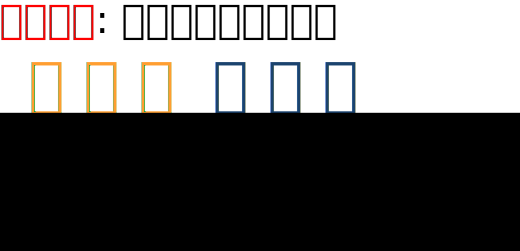
\includegraphics[width=0.75\linewidth]{fig/logogram_and_ideogram.pdf}
    \end{figure}
    \begin{itemize}
      \bigger
      \item モデル: \fire{フォント画像} \arrow 文字埋め込み \\
                    \arrow 単語、文、文書埋め込み \arrow レーティング
    \end{itemize}
  }

  \only<3>{
    \begin{itemize}
      \bigger
      \item 解析結果
    \end{itemize}
    \begin{figure}
      \includegraphics[width=0.8\linewidth]{fig/review_1.png}
    \end{figure}\vspace{-2ex} % HACK
    \begin{figure}
      \includegraphics[width=0.7\linewidth]{fig/review_2.png}
    \end{figure}
  }
\end{frame}

\end{document}
